% Template for ISBI-2018 paper; to be used with:
%          spconf.sty  - ICASSP/ICIP LaTeX style file, and
%          IEEEbib.bst - IEEE bibliography style file.
% --------------------------------------------------------------------------
\documentclass{article}
\usepackage{spconf,amsmath,graphicx}

\usepackage{graphicx,subfigure}
\usepackage{lettrine}
\usepackage{lipsum}
\usepackage{url} 

% Example definitions.
% --------------------
\def\x{{\mathbf x}}
\def\L{{\cal L}}

% Title.
% ------
\title{PECTORAL MUSCLE SEGMENTATION USING WATERSHEDS}
%
% Single address.
% ---------------
\name{Zafar Toshpulatov and Alessandro Bria\thanks{Thanks to Erasmus Mundus Joint Master degree in MAIA for funding.}}
\address{Medical Imaging and Applications, University of Cassino and Southern Latium, Cassino, Italy
}
%
% For example:
% ------------
%\address{School\\
%	Department\\
%	Address}
%
% Two addresses (uncomment and modify for two-address case).
% ----------------------------------------------------------
%\twoauthors
%  {A. Author-one, B. Author-two\sthanks{Thanks to XYZ agency for funding.}}
%	{School A-B\\
%	Department A-B\\
%	Address A-B}
%  {C. Author-three, D. Author-four\sthanks{The fourth author performed the work
%	while at ...}}
%	{School C-D\\
%	Department C-D\\
%	Address C-D}
%
% More than two addresses
% -----------------------
% \name{Author Name$^{\star \dagger}$ \qquad Author Name$^{\star}$ \qquad Author Name$^{\dagger}$}
%
% \address{$^{\star}$ Affiliation Number One \\
%     $^{\dagger}$}Affiliation Number Two
%
\begin{document}
%\ninept
%
\maketitle
%
\begin{abstract}
Breast cancer is the most common cancer among women and digital mammograms are used to detect. When analyzing mammograms with help of an automated computer aided diagnosis system, it can be mistake causing of pectoral muscle. The pectoral muscle segmentation from the breast region is needed for better efficiency. The segmentation of the pectoral muscle is the initial preprocessing step in computer aided diagnosis systems as well as digital mammograms. In this paper, a method for the segmentation of pectoral muscle contour based on contrast enhancement, edge detection and watershed algorithm is proposed. The contrast increases using histogram equalization and the edge detection is implemented by help of gradient magnitude with Sobel filter. The watershed algorithm was used to segment the pectoral muscle. The experimental results on 188 mammogram images from inBreast data base shows that the detection accuracy of the proposed method is 96.4\%.

\end{abstract}
%
\begin{keywords}
Breast segmentation, Pectoral muscle, Mammogram, Watersheds, Medical Imaging
\end{keywords}
%
\section{Introduction}
\label{sec:intro}
\lettrine[findent=2pt]
{\fbox{\textbf{I}}}{}n 2018, it is estimated to have 266,120 new cases of women invasive breast cancer in addition to 63,960 noninvasive cases in the U.S \cite{2}. After cardiovascular diseases, breast cancer is the leading tumor among women in Italy \cite{1}, whereas in the European Union it is responsible for one in every six deaths from cancer in women \cite{3}. In order to control this alarming mortality rate associated with breast cancer, mass screening is recommended by the medical community world wide. Mammography is a widely-used X-ray imaging modality for breast cancer screening. 

In order to detect and classify the breast cancer, Computer Aided Diagnosis (CAD) systems have been developed. When analyzing mammograms with help of CAD system, it can be mistake causing of pectoral muscle. The pectoral muscle segmentation from the breast region is needed for better efficiency. The segmentation of the pectoral muscle is the initial preprocessing step in computer aided diagnosis systems. The pectoral muscle is always located in the upper left or right region of the mammogram which is a compact and fairly homogeneous region whose average intensity is higher than the breast as described in Figure \ref{fig:mammogram}.

\begin{figure}[h!]
    \centering
    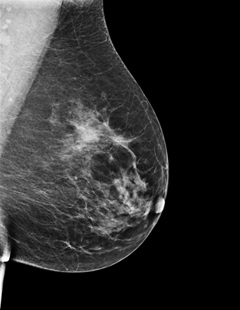
\includegraphics[width=0.25\textwidth]{images/breast.jpg} 
    \caption{Mammogram image}
    \label{fig:mammogram}
\end{figure}  

The main objective of this work is to develop a reusable module for automated pectoral muscle segmentation for further analysis. An effective automated computer approach is presented for pectoral muscle segmentation technique based on contrast enhancement, edge detection and watershed algorithm. The contrast is enhanced using histogram equalization and the edge detection is implemented by help of gradient magnitude with Sobel filter. The watershed algorithm is used to segment the pectoral muscle. The paper consists of three section which are: materials and method, results and discussion, conclusion and future work.

\section{MATERIALS and METHOD}
\label{sec:mat_and_meth}

In this paper, 188 mammogram images were used from INBREAST dataset which contains images of size 3328x4084 and 2560x3328 with 16 bits per pixel. The implementation of the proposed method was carried out on MATLAB 2015b environment. The block diagram in Figure \ref{fig:block_diag} describes all the steps during the implementation of the proposed method. The proposed method consists of two main steps: preprocessing and segmentation based on watersheds \cite{6}.

\subsection{Preprocessing}
\label{ssec:Preprocessing}

The mammogram images were preprocessed in the following steps:
 
\subsubsection{Histogram equalization}
\label{sssec:hist_eq}

The contrast of pectoral muscle contour was enhanced using histogram equalization [2], as shown in Figure \ref{fig:b}. This technique will increase the intensity of pectoral muscle and the contrast of background noise.

\subsubsection{Gaussian smoothing}
\label{sssec:gaus_smooth}

To remove the noise of image, low pass Gaussian smoothing filter was applied to blur with standard deviation of 12 (sigma), as shown in Figure \ref{fig:c}.

\subsubsection{Edge detection using gradient magnitude}
\label{sssec:grad_mag}

The gradient is high at the border of the pectoral muscle and low inside. To detect the edge of pectoral muscle, gradient magnitude was computed using vertical and horizontal derivatives with Sobel operator as described in Figure \ref{fig:d}.

\begin{figure}[h!]
    \centering
    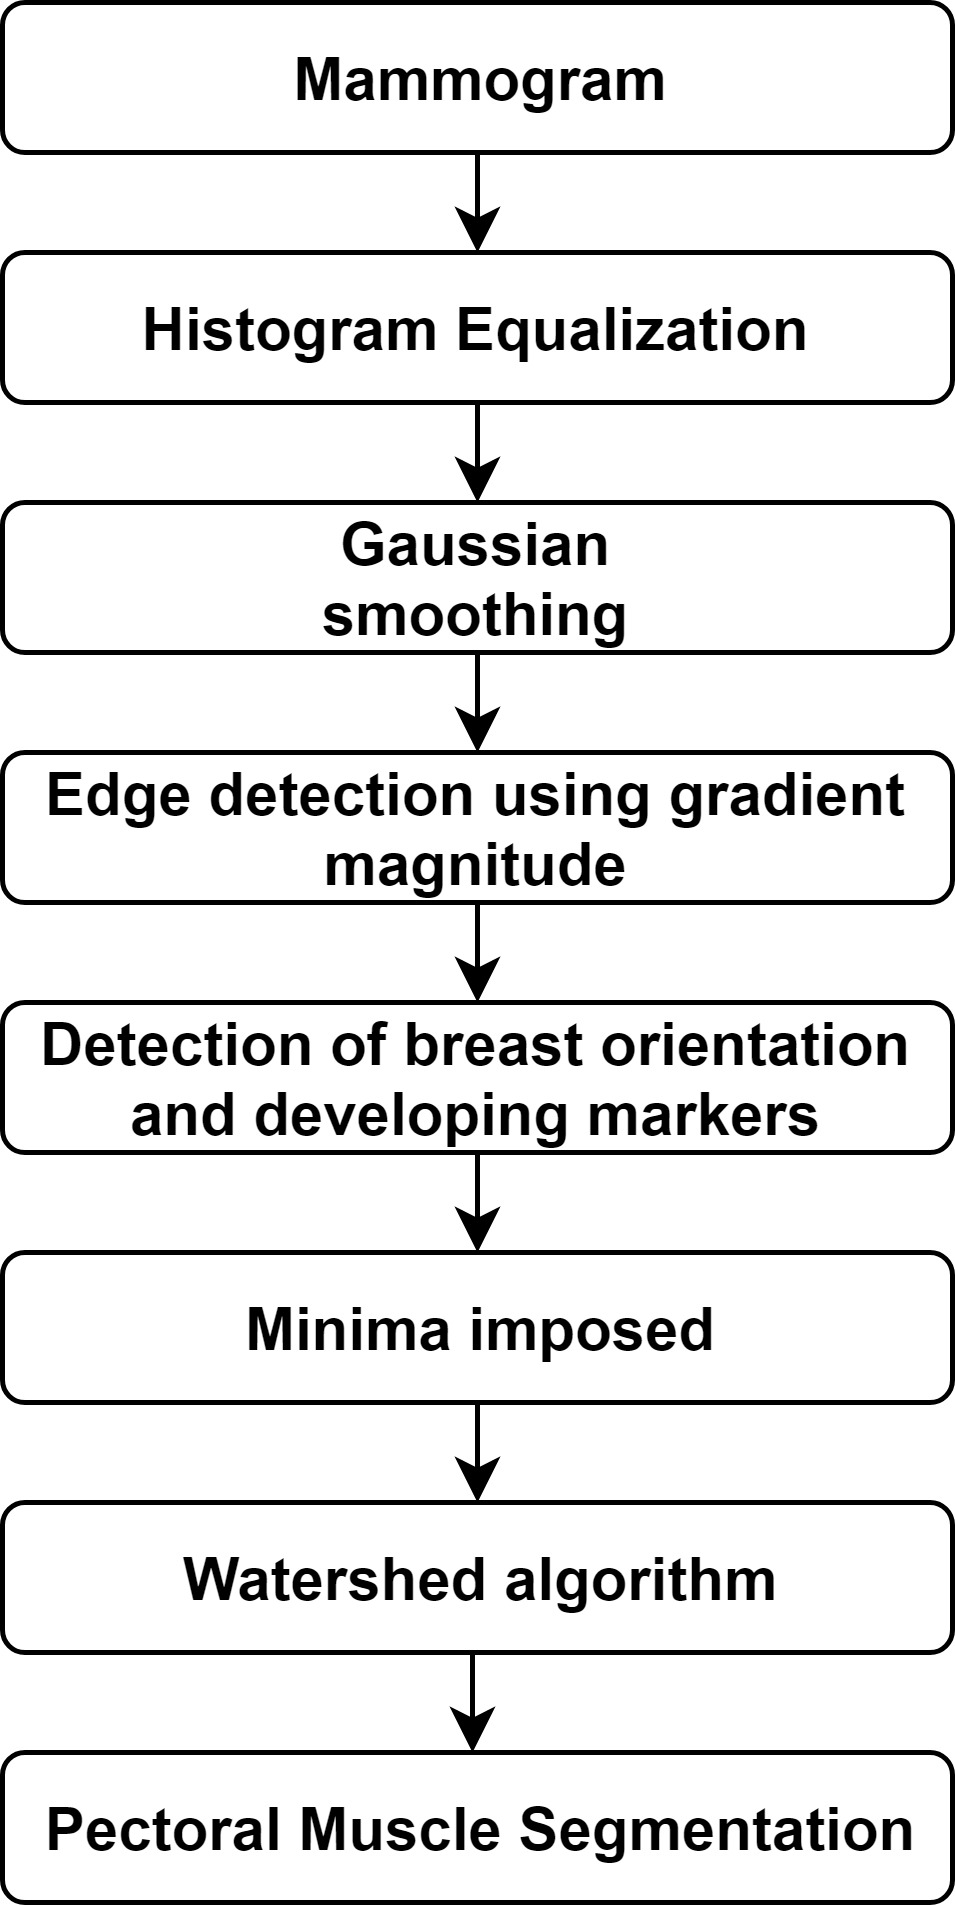
\includegraphics[width=0.25\textwidth]{images/block_diag.jpg} 
    \caption{Block diagram}
    \label{fig:block_diag}
\end{figure} 

\subsection{Segmentation based on watersheds}
\label{ssec:segmen_water}

\subsubsection{Detection of breast orientation and developing markers}
\label{sssec:orien_marker}

The mammogram images contain the left and right breast and it should be classified as left or right pectoral muscle. The orientation of breast was detected by checking the intensity pixel of top left corner. Once the orientation is known, in Figure \ref{fig:e} two markers were created as internal (pectoral muscle) and external (breast region) markers with white foreground and black background for further watershed implementation. If breast is oriented as right, the markers are flipped otherwise it will continue the subsequent operation .

\subsubsection{Minima imposed and Watershed algorithm}
\label{sssec:grad_mag}

These two markers were imposed on gradient magnitude image to obtain the minima for Watershed transformation so that it has regional minima only in certain desired locations as shown in Figure \ref{fig:f}. \cite{6} Watershed algorithm was used to divide minima imposed image into two regions. The gradient image can be viewed topographic surface where higher intensities represent hills (gradient) and lower intensities represent valleys (minima). The water rises from the minimum point of valleys and fills the holes. \cite{7} The filling of water and building of bariers continue until all the peaks are under water. The borders between different water sources gives segmentation result as described in Figure \ref{fig:watershed}.

 \begin{figure}[h!]
    \centering
    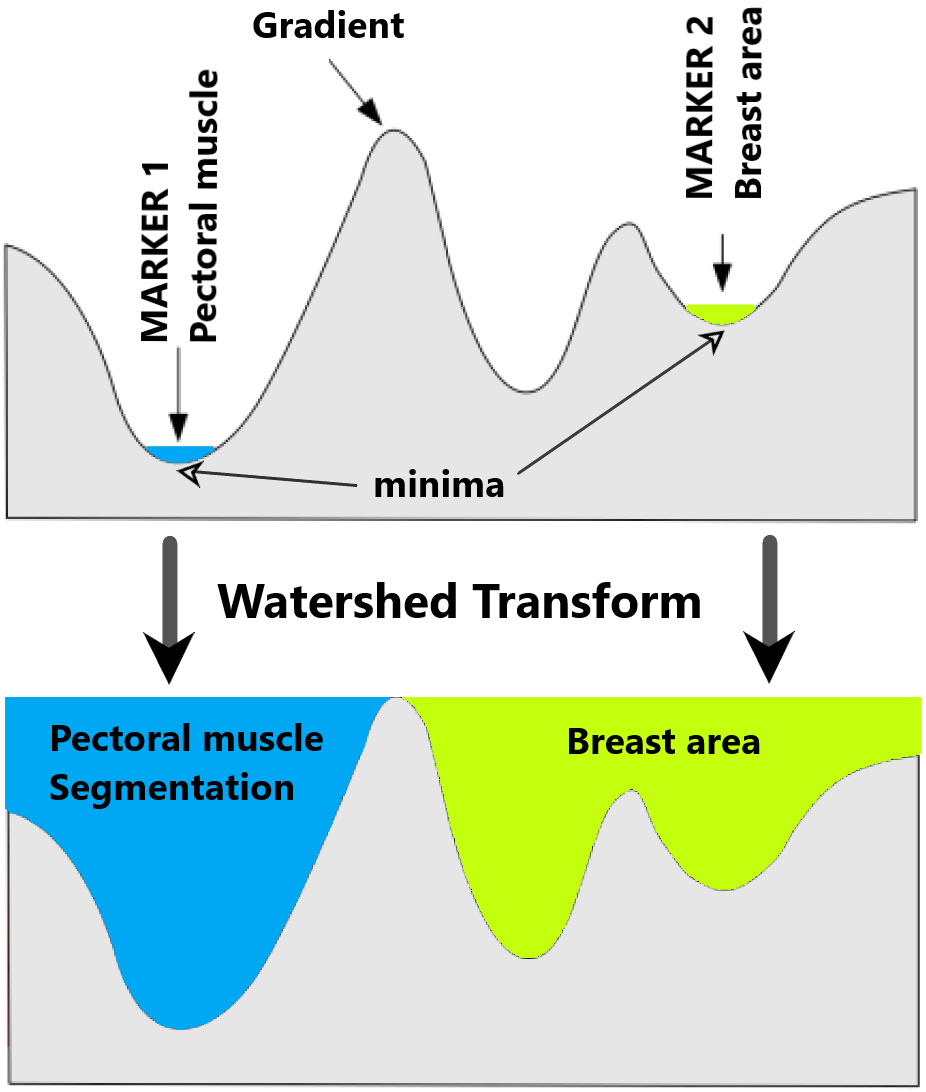
\includegraphics[width=0.40\textwidth]{images/watershed_algorithm.png} 
    \caption{Watershed algorithm}
    \label{fig:watershed}
\end{figure} 

\begin{figure}
\centering     %%% not \center
\subfigure[Mammogram]{\label{fig:a}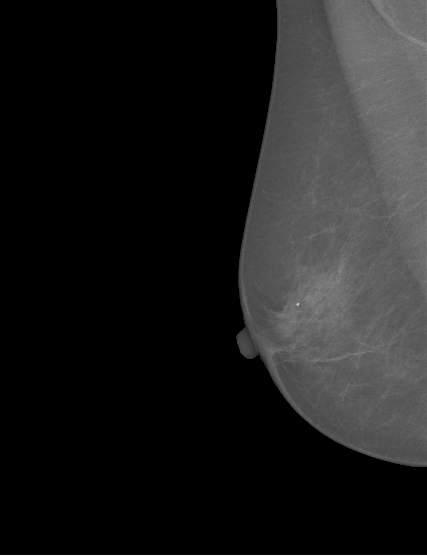
\includegraphics[width=36mm]{images/original.png}}
\subfigure[Histogram equalization]{\label{fig:b}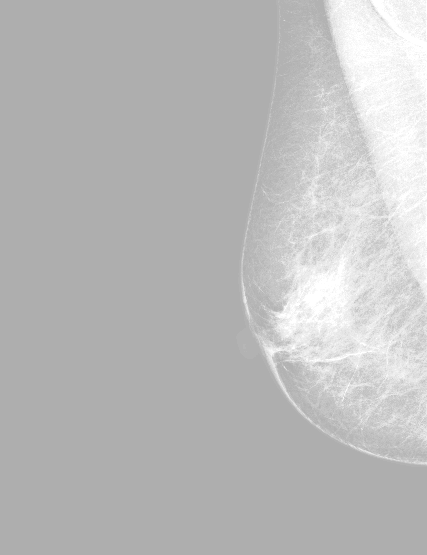
\includegraphics[width=36mm]{images/hist_eq.png}}
\subfigure[Gaussian smoothing]{\label{fig:c}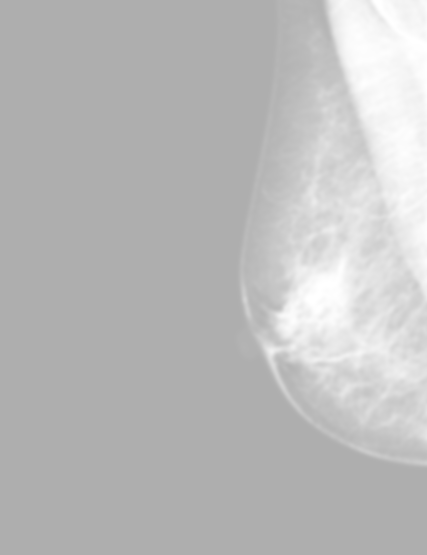
\includegraphics[width=36mm]{images/gauss_smooth.png}}
\subfigure[Edge detection using gradient magnitude]{\label{fig:d}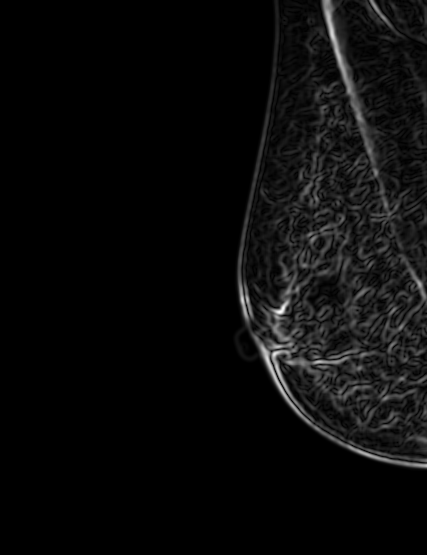
\includegraphics[width=36mm]{images/grad_mag.png}}
\subfigure[Detection of  breast orientation and developing markers]{\label{fig:f}
\includegraphics[width=36mm]{images/markers.png}}
\subfigure[Minima imposed]{\label{fig:e}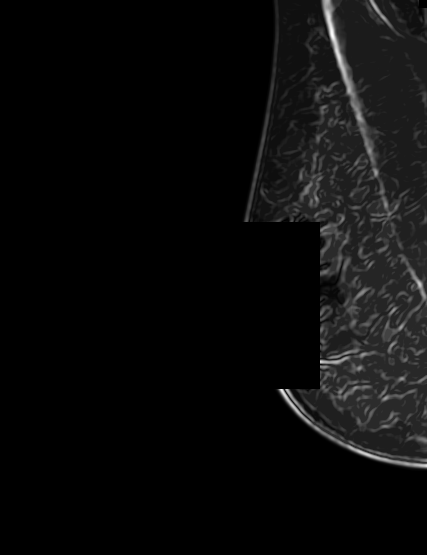
\includegraphics[width=36mm]{images/impose_minima.png}}
\subfigure[Pectoral Muscle Segmentation after watershed transformation]{\label{fig:g}
\includegraphics[width=36mm]{images/pectoral_muscle.png}}
\caption{Step of the proposed method}
\end{figure}


\section{RESULTS AND DISCUSSION}
\label{sec:res_discuss}

After processing the mammogram images using the adopted method, the segmented pectoral muscle was obtained from each image. In order to evaluate the performance of the method for pectoral muscle segmentation, the accuracy (ACC) was defined using the breast air mask and ground truth as given in Equation \ref{eq:acc}.

    \begin{equation}\label{eq:acc}
       ACC = \frac{TP + TN}{Total\; number\; of\; samples}
    \end{equation}

TP (True Positive) are the pixels that were correctly segmented as pectoral muscle, TN (True Negative) are the pixels that were falsely segmented as pectoral muscle and total number of samples (pixels of the mask).

As a result, the detection accuracy of the proposed method was 96.4\% for 188 mammogram images. Based on the visual analysis of the obtained results, it was observed that most of the images (132 images, 70\%) were segmented correctly by the proposed method. 26 images (in 13\% cases) gave acceptable segmentation. However, the 32 images (17\%) that reflected bad performance is shown in Figure \ref{fig:bad_segment} where the pectoral muscle is not covered due to its two edges.

 \begin{figure}[h!]
    \centering
    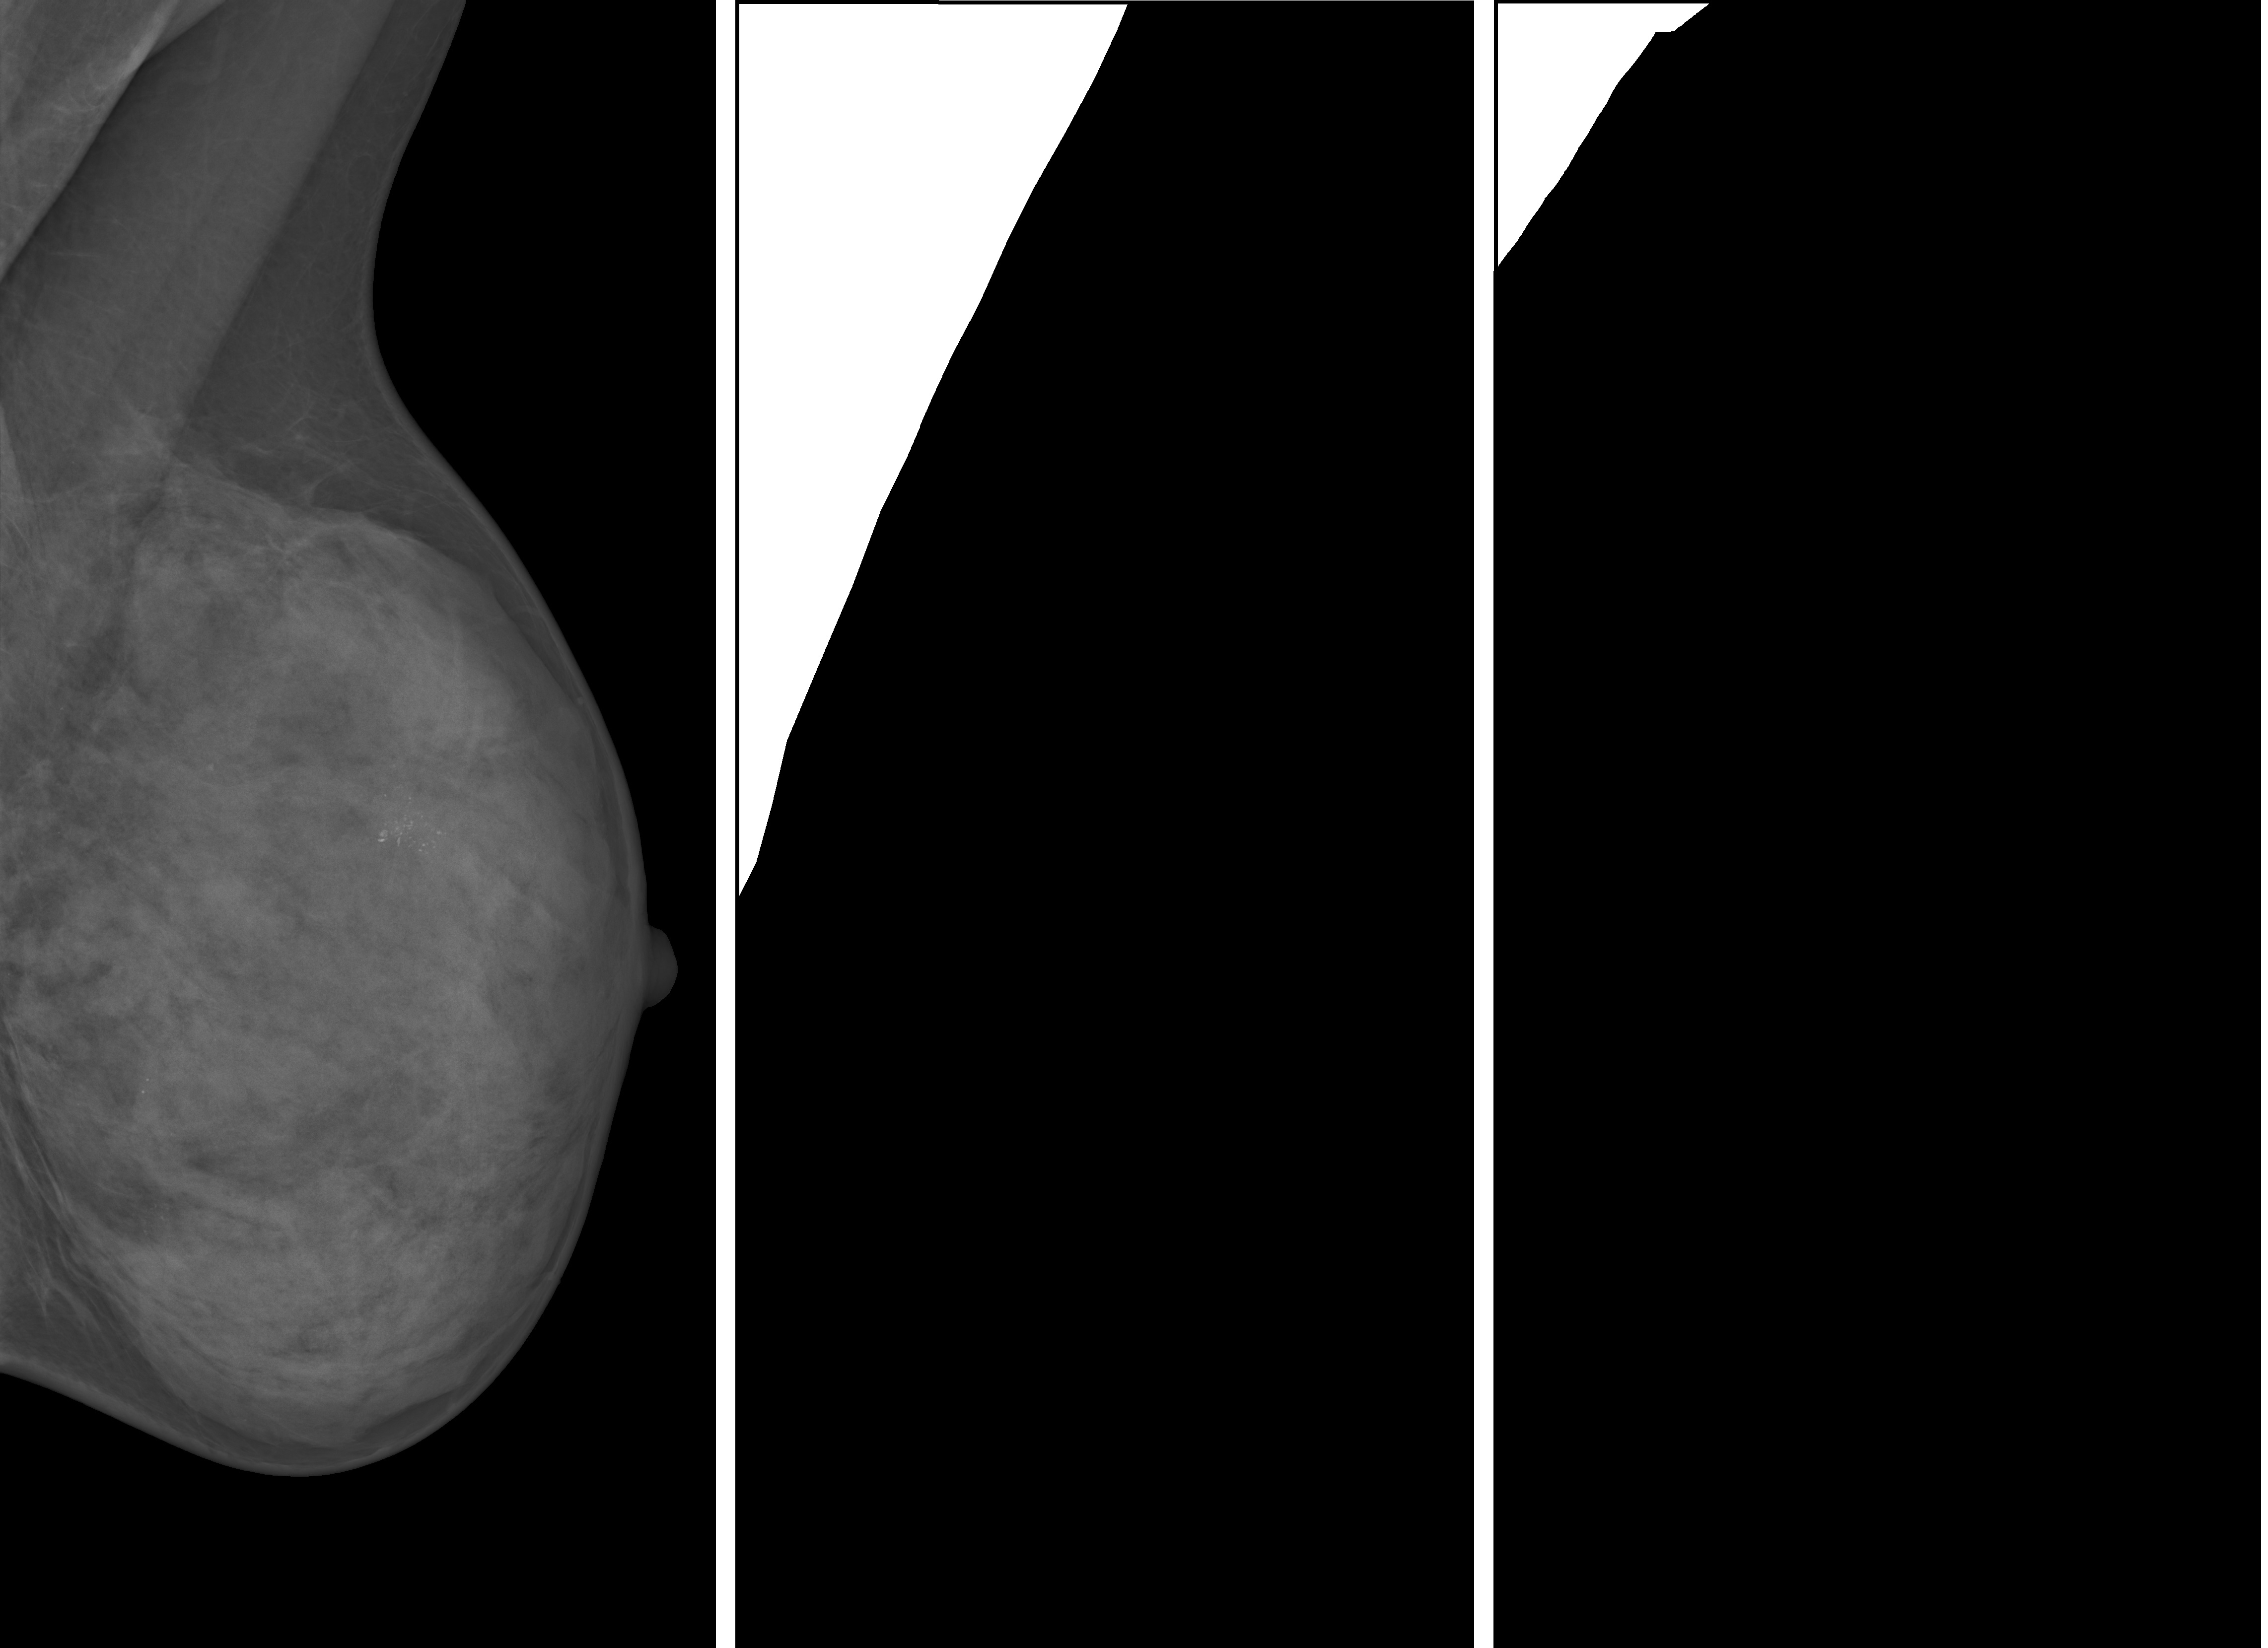
\includegraphics[width=0.45\textwidth]{images/bad_segment.jpg} 
    \caption{Bad pectoral muscle segmentation. Comparison mammogram, ground truth and segmented images.}
    \label{fig:bad_segment}
\end{figure} 

Unfortunately, this method has some problems that the pectoral muscle contour is not always detected cause of the created markers is not include the pectoral muscle. Sometimes, the intensity of pectoral muscle and breast profile boundaries are very similar and both boundaries are blended. In addition, it is not always usefull to manually place a marker in the breast profile.

% To start a new column (but not a new page) and help balance the last-page
% column length use \vfill\pagebreak.
% -------------------------------------------------------------------------
%\vfill
%\pagebreak


\section{CONCLUSION AND FUTURE WORK}
\label{sec:conclusion}

In this paper, an effective automated computer approach was presented for pectoral muscle segmentation technique with help of image processing and watershed algorithm. The efficiency of the method was tested on 188 mammogram images  taken from the inBreast database. However, finding an approach that can detect the border of the pectoral muscle  proved to be a difficult task. The main problem was to find properly pectoral muscle edge. As some mammogram images have two or three boundaries. Furthermore some region in breast profile has the similar intensity of pectoral muscle boundary. It is observed that the performance of the pectoral muscle segmentation can be improved by the help of curve fitting the edge of the pectoral muscle, to be segmented the similar intensity boundaries and counting the boundaries of the pectoral muscle \cite{7}.

% References should be produced using the bibtex program from suitable
% BiBTeX files (here: strings, refs, manuals). The IEEEbib.bst bibliography
% style file from IEEE produces unsorted bibliography list.
% -------------------------------------------------------------------------
%\bibliographystyle{IEEEbib}
%\bibliography{strings,refs}

\begin{thebibliography}{5}
    
	%Each item starts with a \bibitem{reference} command and the details thereafter.
	\bibitem{1}
	Annuario Statistico. Italian National Institute of Statistics. {\em Italiano},
	2002.
    
    \bibitem{2}
	U.S. Breast Cancer Statistics. \url{https://www.breastcancer.org/symptoms/understand_bc/statistics},

    \bibitem{3}
	L. Eurostat. Health statistics Atlas on mortality in the European Union. ser. International series of monographs on physics. Luxembourg: Office for Official Publications of the European Communities, 2009.
	
	\bibitem{4}
	Hanan Alshanbari, Saad Amain, James Shuttelworth,Khaled Slman and Shadi Muslam. AUTOMATIC SEGMENTATION IN BREAST CANCER USING WATERSHED ALGORITHM. {\em International Journal of Biomedical Engineering and Science (IJBES)} Faculty of Engineering and Computing, Coventry University, Vol. 2, No. 2, April 2015
	
	\bibitem{5}
	Woong Bae Yoon, Ji Eun Oh, Eun Young Chae, Hak Hee Kim, Soo Yeul Lee, and Kwang Gi Kim, “Automatic Detection of Pectoral Muscle Region for Computer-Aided Diagnosis Using MIAS Mammograms,”   {\em BioMed Research International}, vol. 2016, Article ID 5967580, 6 pages, 2016.  \url{https://doi.org/10.1155/2016/5967580}.

	\bibitem{6}
	Marker-Controlled Watershed Segmentation, \url{https://fr.mathworks.com/help/images/examples/marker-controlled-watershed-segmentation}

	\bibitem{7}
Fernand Meyer, “Topographic distance and watershed lines,”  {\em Signal processing}, vol. 38, no. 1, pp. 113–125, 1994.

\end{thebibliography}

\end{document}
